\section{Νευρωνικά Δίκτυα με Βάθος}
\label{sec:theory_dnn}

Τα Νευρωνικά Δίκτυα είναι εμπνευσμένα από το βιολογικό νευρικό σύστημα του
του ανθρώπου. Η βασική επεξεργαστική μονάδα του εγκεφάλου είναι ο \emph{νευρώνας}.
Το ανθρώπινο νευρικό σύστημα αποτελείτε από περίπου 86 εκατομμύρια νευρώνες και περίπου
$10^14 - 10^15$ διασυνδέσεις.
\begin{figure}[!ht]
  \centering
  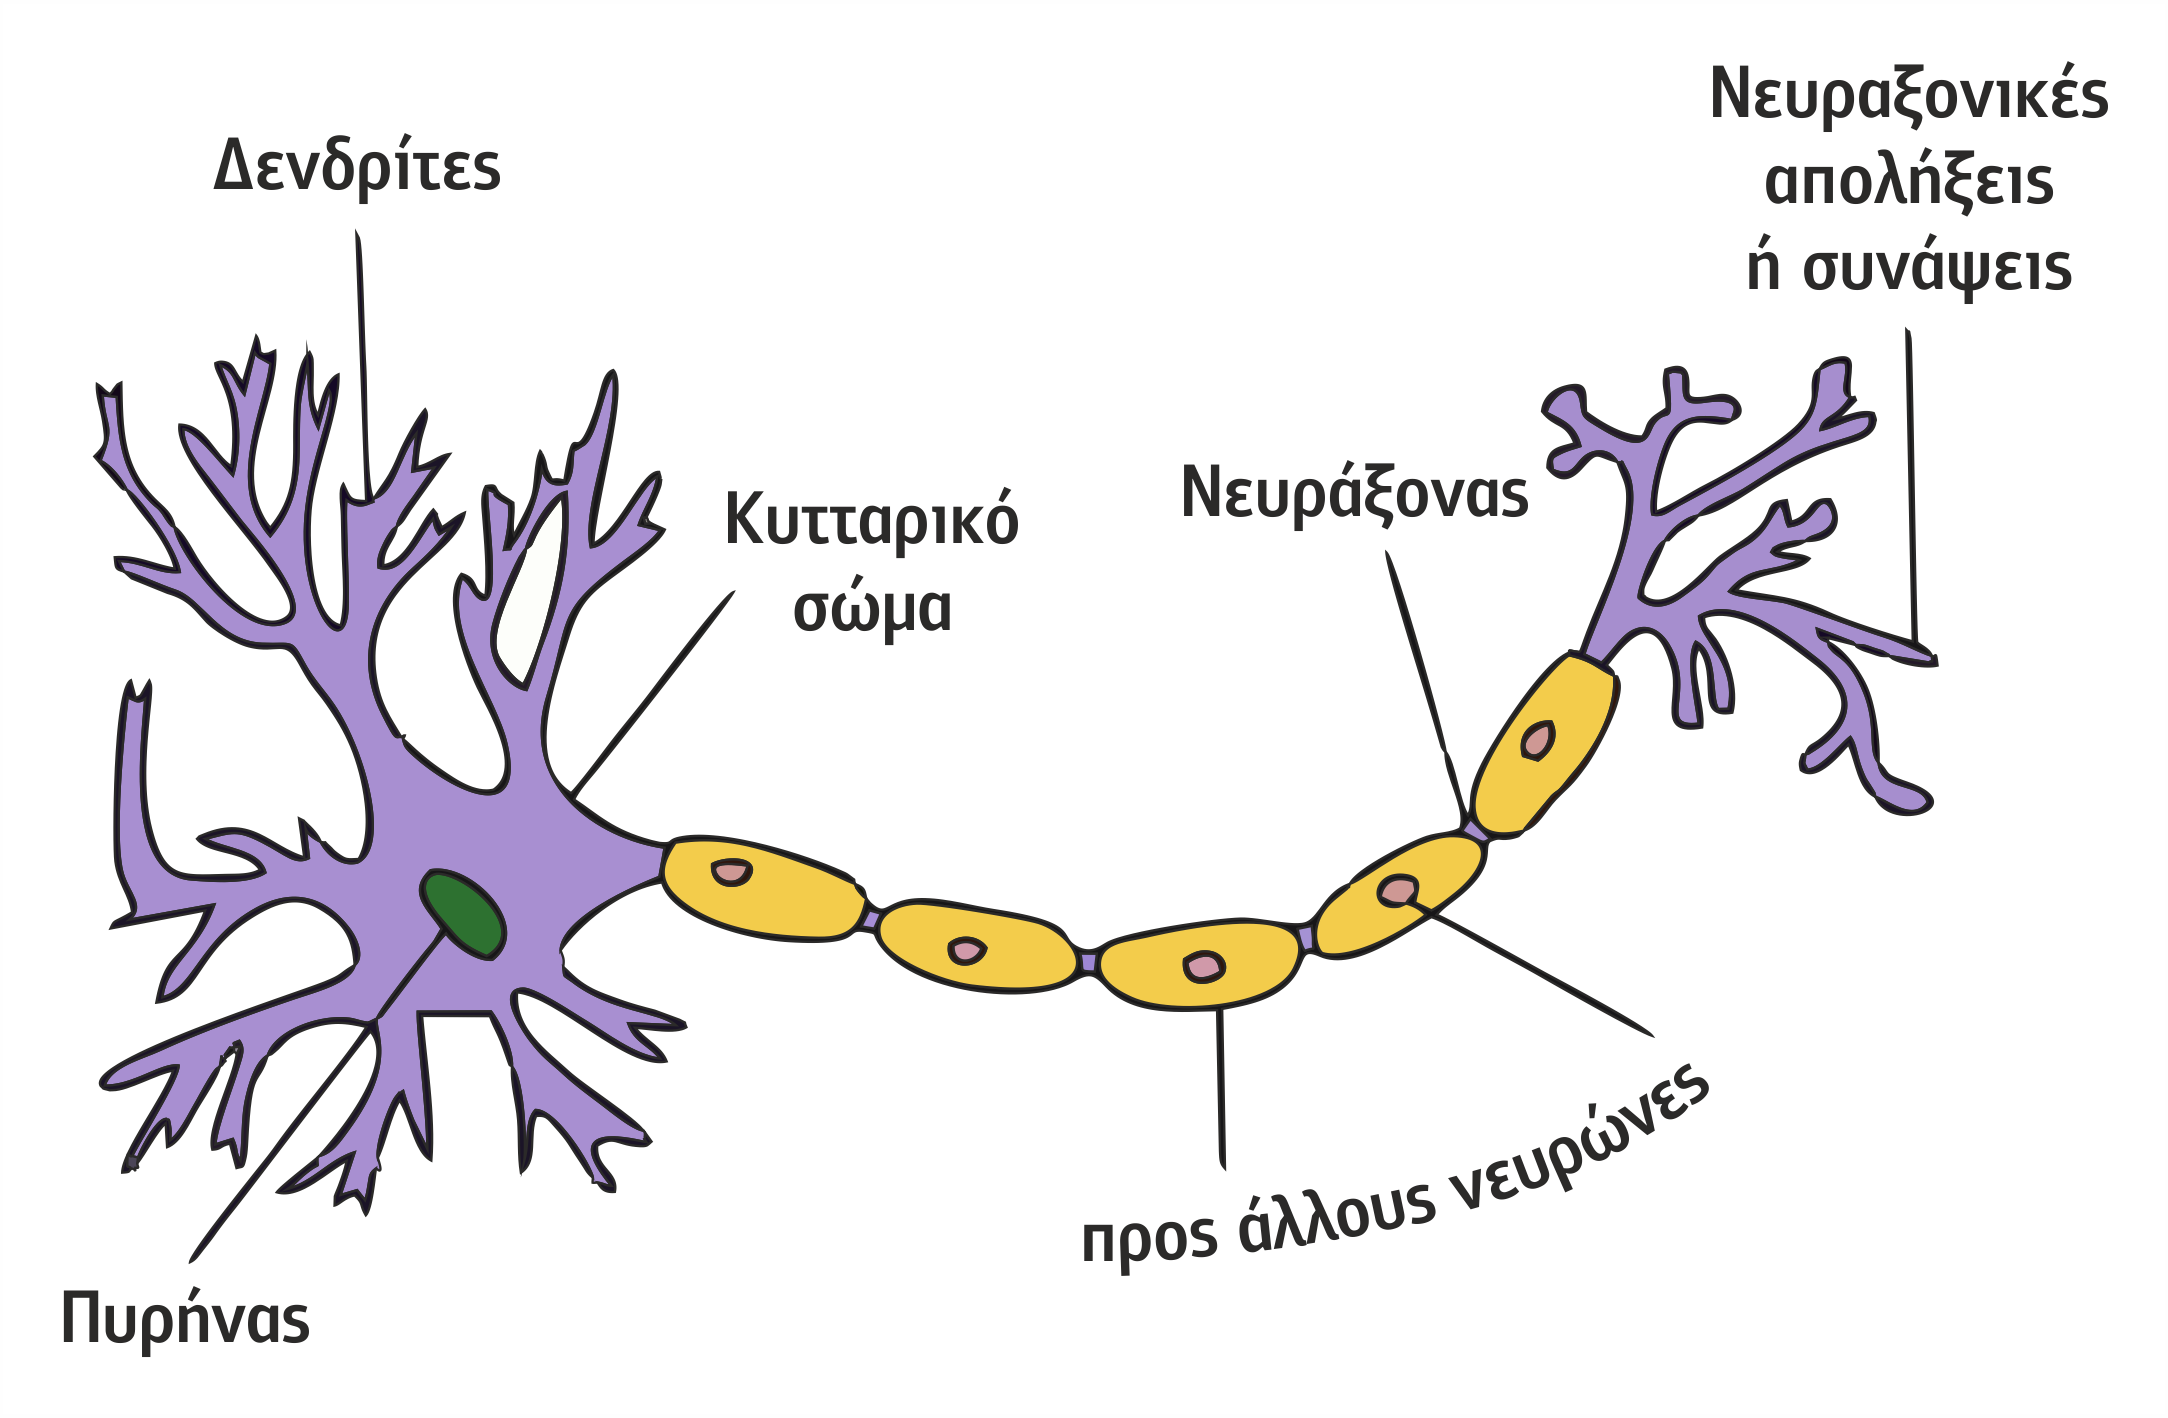
\includegraphics[width=0.7\textwidth]{./images/chapter3/neuron.png}
  \caption[Βιολογικός Νευρώνας]{Βιολογικός νευρώνας.}
  \label{fig:neuron_bio}
\end{figure}
Στο \autoref{fig:neuron_bio} φαίνεται η μορφή και tα μέλη ενός βιολογικού νευρώνα
Τα κύρια μέρη ενός νευρώνα είναι τα εξής:
\begin{itemize}
  \item{\textbf{Δενδρίτης (Dendrites)}: Δέχεται είσοδο από άλλους νευρώνες.}
  \item{\textbf{Σώμα του κυττάρου (Cell body)}: Εξάγει συμπεράσματα, με βάση τις εισόδους.}
  \item{\textbf{Νευράξονας (Axon)}: Συνδέει την έξοδο που λαμβάνεται από το σώμα του κυττάρου με τις νευρωνικές απολήψεις}
  \item{\textbf{Νευραξονικές απολήψεις}: Συνδέει τον νευράξονα του εκάστοτε νευρώνα με τους τερματικόυς κόμβους
    από όπου και μεταφέρεται η πληροφορία σε άλλους νευρώνες.
    είσοδο άλλων νευρώνων.}
\end{itemize}
Κάθε νευρώνας δέχεται είσοδο από άλλους νευρώνες μέσω των δενδρίτων του.
Στην συνέχεια επεξεργάζεται το σήμα που λαμβάνει στην είσοδο και
στέλνει το αποτέλεσμα στον νευράξονα. Τέλος άλλοι νευρώνες συνδέονται με αυτόν
μεσω των συνάψεων του.

\begin{figure}[!ht]
  \centering
  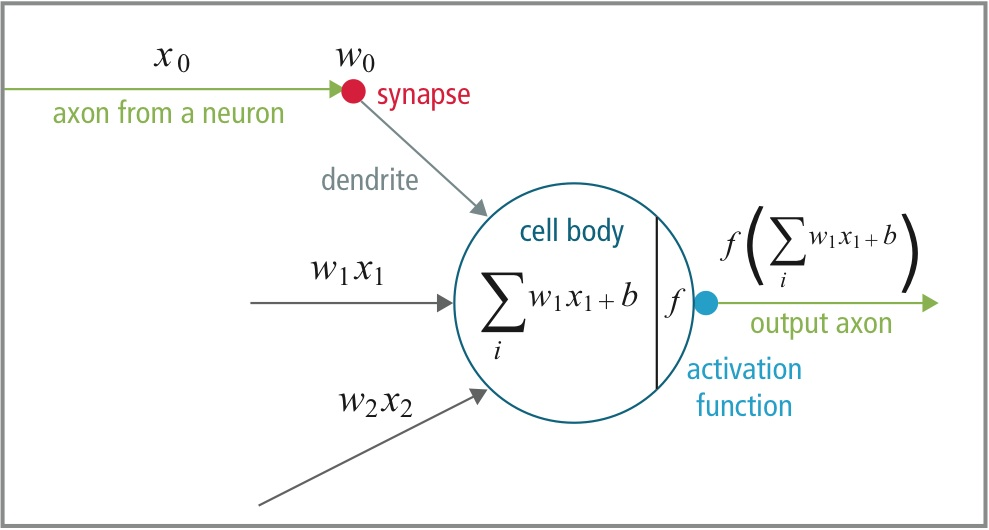
\includegraphics[width=0.7\textwidth]{./images/chapter3/neuron_model.jpg}
  \caption[Μαθηματικό μοντέλο του νευρώνα]{Μαθηματικό μοντέλο του νευρώνα}
  \label{fig:neuron_model}
\end{figure}

To αντίστοιχο μαθηματικό μοντέλο του νευρώνα, φαίνεται στο \autoref{fig:neuron_model}.
H πληροφρία που μεταφέρεται από τις νευραξονικές απολήψεις ($x0$), πρωτού
στους δενδρίτες των επόμενων νευρώνων, αλληλεπιδρά πολλαπλασιαστικά με τις
συνάψεις ($w0*x0$). Oι πολλαπλασιστικοί παράγωντες $w_n$ ονομάζονται βάροι
και αποτελούν τις μεταβλητές παραμέτρους ενός νευρώνα. Η τιμή των παραμέτρων
αυτών ελέγχουν την επίδραση μεταξύ των νευρώνων. Η συνάρτηση ενεργοποίησης $f$
ελέγχει την ροή της πληροφορίας στους συνδεδεμένους νευρώνες,
και προσδίδει ευελιξία και ικανότητα εκτίμησης όσον αφoρά πολύπλοκες μή γραμμικές
σχέσεις στα δεδομένα εισόδου.
Η πιο συχνά χρησιμοποιούμενη και απλή στην λειτουργία συνάρτηση ενεργοποίησης
είναι η σιγμοειδής συνάρτηση $\sigma(x) = 1 / (1 + e^{-x})$.
Εναλλακτικά, η σιγμοειδές συνάρτηση ενεργοποίησης μπορει να εκφραστει σε διακριτή μορφή ως
\[
f(x) =
  \begin{cases}
    0, & x < 0 \\
    1, & x \geq 0 \\
  \end{cases}
\]

Γενικότερα, ο νευρώνας μπορεί να είναι και πολωμένος (bias - $b$) και έτσι το μαθηματικό
μοντέλο που τον περιγράγει πλήρως παίρνει την μορφή:
\begin{center}
\begin{large}
  $f(\sum_{\imath} \vec{X_{\imath}}\vec{W_{\imath}} + b) = \frac{1}{1 + e^{-\sum_{\imath} \vec{X_{\imath}}\vec{W_{\imath}} + b}}$
\end{large}
\end{center}
Θα μπορούσαμε να ερμηνεύσουμε το αποτέλεσμα της εφαρμογής της
σιγμοειδή συνάρτηση ενεργοποίησης ώς την πιθανότητα μίας από τις κλασεις:
\begin{center}
\begin{large}
  $P(y_{\imath} = 1 | x_{\imath};w)$ \\
  $P(y_{\imath} = 0 | x_{\imath};w) = 1 - P(y_{\imath} = 1 | x_{\imath};w)$
\end{large}
\end{center}

Σαν παρατήρηση, με εφαρμογή κατάλληλης
συνάρτησης σφάλματος στην έξοδο, ο νευρώνας μετατρέπεται σε ένα  γραμμικό ταξινομητή
(linear classifier). Πιο συγκεκριμένα, σε περίπτωση που χρησιμοποιήσουμε την \emph{cross-entropy}
συνάρτηση σφάλματος ο νευρώνας μετατρέπεται σε δυαδικό ταξινομητή \textbf{Softmax},
τον οποίο και θα συναντήσουμε στην συνέχεια.

\begin{figure}[!ht]
  \centering
  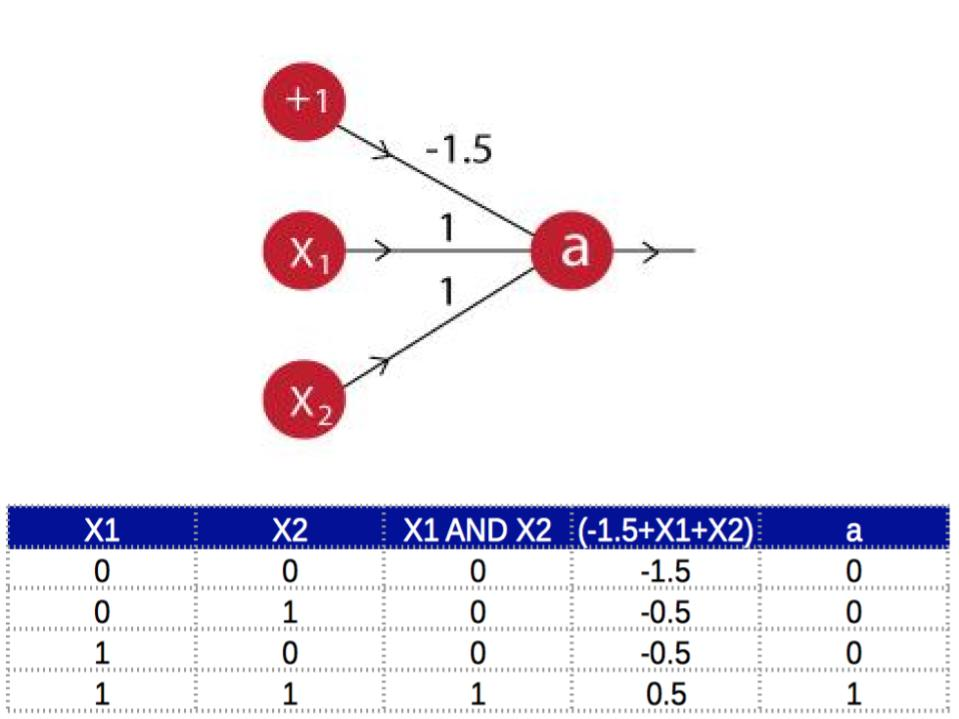
\includegraphics[width=0.6\textwidth]{./images/chapter3/perceptron_and.jpg}
  \caption[Υλοποίηση πύλης AND με χρήση του μαθηματικού μοντέλου του perceptron]{Υλοποίηση πύλης AND με χρήση του μαθηματικού μοντέλου του perceptron}
  \label{fig:neuron_and}
\end{figure}

Μία από τις τρεις θεμείώδεις εφαρμογές του μαθηματικού μοντέλου του νευρώνα είναι η υλοποίηση της
δυαδικής πράξης \textbf{AND}, η οποία και φαίνεται στο \autoref{fig:neuron_and}.
Οι άλλες δύο είναι προφανώς οι πράξεις \textbf{OR} και \textbf{NOT}.

H σύνδεση πολλών νευρώνων σε σε έναν γράφο δομεί ένα \emph{Νευρωνικό Δίκτυο},
το οποίο έχει την μορή του σχήματος \autoref{fig:simple_nn}.
To συγκεκριμένο μοντέλο ΝΝ ονομάζεται \emph{Perceptron} ή αλλιώς
\emph{Feedforward Artificial Neural Network}, ο οποίος έχει τα εξής χαρακτηριστικα:
\begin{itemize}
  \item{Οι διασυνδέσεις μεταξύ των νευρώνων δεν σχηματίζουν σε καμία περίπτωση κύκλο.}
  \item{Αποτελείτε από 2 επίπεδα; ένα κρυφό επίπεδο και το επίπεδο εξόδου}
  \item{Χρησιμοποιείται η σιγμοειδή συνάρτηση ενεργοποίησης}
\end{itemize}

Τα μοντέλα ΝΝ συχνά οργανώνονται σε διακριτά επίπεδα από νευρώνες, όπου οι
νευρώνες που ανήκουν σε ένα επίπεδο συνδέονται με νευρώνες του
προηγούμενου και του επόμενου επιπέδου. Όσον αφορά την αρίθμηση
των επιπέδων ενός νευρωνικού δικτύου, αναφέρουμε ότι συμβατικά το πρώτο επίπεδο
δεν υπολογίζεται αφού πρακτικά αποτελεί τα ίδια τα δεδομένα εισόδου.

\begin{figure}[!ht]
  \centering
  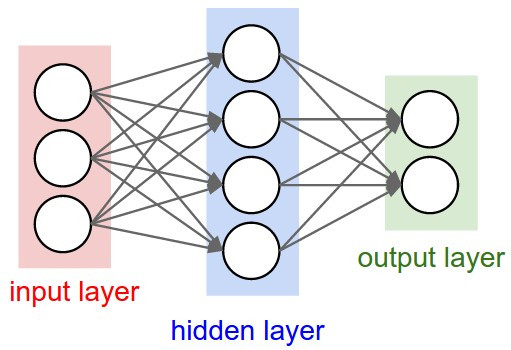
\includegraphics[width=0.5\textwidth]{./images/chapter3/simple_nn.jpg}
  \caption[Απλό μοντέλο NN με ένα κρυφό επίπεδο]{Απλό μοντέλο NN με ένα κρυφό επίπεδο}
  \label{fig:simple_nn}
\end{figure}

Η επιλογή εφαρμογής της σιγμοειδής συνάρτησης, ως συνάρτηση ενεργοποίησης των
νευρώνων που αποτελούν ένα ΝΝ δεν είναι τυχαία, αφού όπως θα δούμε στην
συνέχεια επιτρέπει την εφαρμογή του αλγορίθου \emph{Backpropagation} για την
εκπαίδευση των νευρωνικών δικτύων.

\begin{algorithm}[!htp]
  \caption{Υπολογισμός εξόδων ενός ΝΝ}
  \label{alg:nn_forward}
  \begin{algorithmic}[1]
    \Procedure {nn\_forward}{X, W, B, num\_layers}
      \State $k \gets 0$
      \While{$k < num\_layers$}
        \State $X \gets 1 / (1 + e^{-\sum_{\imath} X \odot W_{k} + B_{k}})$
        \State $k \gets k+1$
      \EndWhile
    \EndProcedure
  \end{algorithmic}
\end{algorithm}

O \autoref{alg:nn_forward} υλοποιεί την συνάρτηση για τον υπολογισμό της εξόδου
ενός νευρωνικού δικτύου (forward pass), έχοντας σαν δεδομένα τα βάρη και τις τιμές της πόλωσης
των νευρώνων του κάθε επιπέδου, καθώς και τα δεδομένα εισόδου.


\subsection{Συναρτήσεις Ενεργοποίησης}

TODO!

\subsection{Ο αλγόριθμος Backpropagation}

TODO!

\subsection{Αρχιτεκτονικές}

TODO!
